\chapter{Literature Review and Definitions}
\label{sec:background}

This chapter presents the concepts and theory required to understand the methodology, rationale and contributions of this dissertation. It starts by defining a Cognitive Architecture, and goes into more detail about Adaptive Control of Thought - Rational (ACT-R), which is the underlying framework used in the Integrated Driver Modelling described in Section \ref{sec:salvucci} and the basis for the system developed in Chapter 3. The chapter concludes with the introduction of several important concepts in the area of Probabilistic Model Checking, which are essential for modelling, verification and synthesis in this context.

\section{Cognitive Architectures}

Different definitions of a cognitive architecture can be found in the literature \cite{cog_arch_1}. According to Sun, a cognitive architecture is a \textit{"broadly-scoped, domain-generic computational cognitive model, capturing the essential structure and process of the mind, to be used for a broad, multiple-level, multiple-domain analysis of behavior"} \cite{cog_arch_2}. In that sense, a cognitive architecture is no more than a formalised framework of the perception, memorisation, decision making, reasoning and execution of the human mind. It is important to note that this architecture should capture both the abilities (e.g. memory storage and recall, perception or motor action) and constraints (e.g. memory decay and limited motor performance) of the human system \cite{salvucci_1}.

The idea of a cognitive architecture originated in the early 1970s. A survey by Korseruba and Tsotsos  \cite{cog_arch_1} revealed that, since then, an estimated 195 different cognitive architectures with different assumptions, structural organisations and implementations have been developed. Applications of these range from the fields of Robotics to Natural Language Processing \cite{cog_arch_1}. One of the most well known of those architectures is Adaptive Control of Thought - Rational.

\subsection{Adaptive Control of Thought - Rational (ACT-R)}

Adaptive Control of Thought - Rational (or ACT-R as it is commonly known as) is a particular cognitive architecture first presented by John R. Anderson in 1983 \cite{actr_1} and further developed by Anderson \textit{et al.} in \cite{actr_2}. 

\begin{figure}[h]
    \centering
    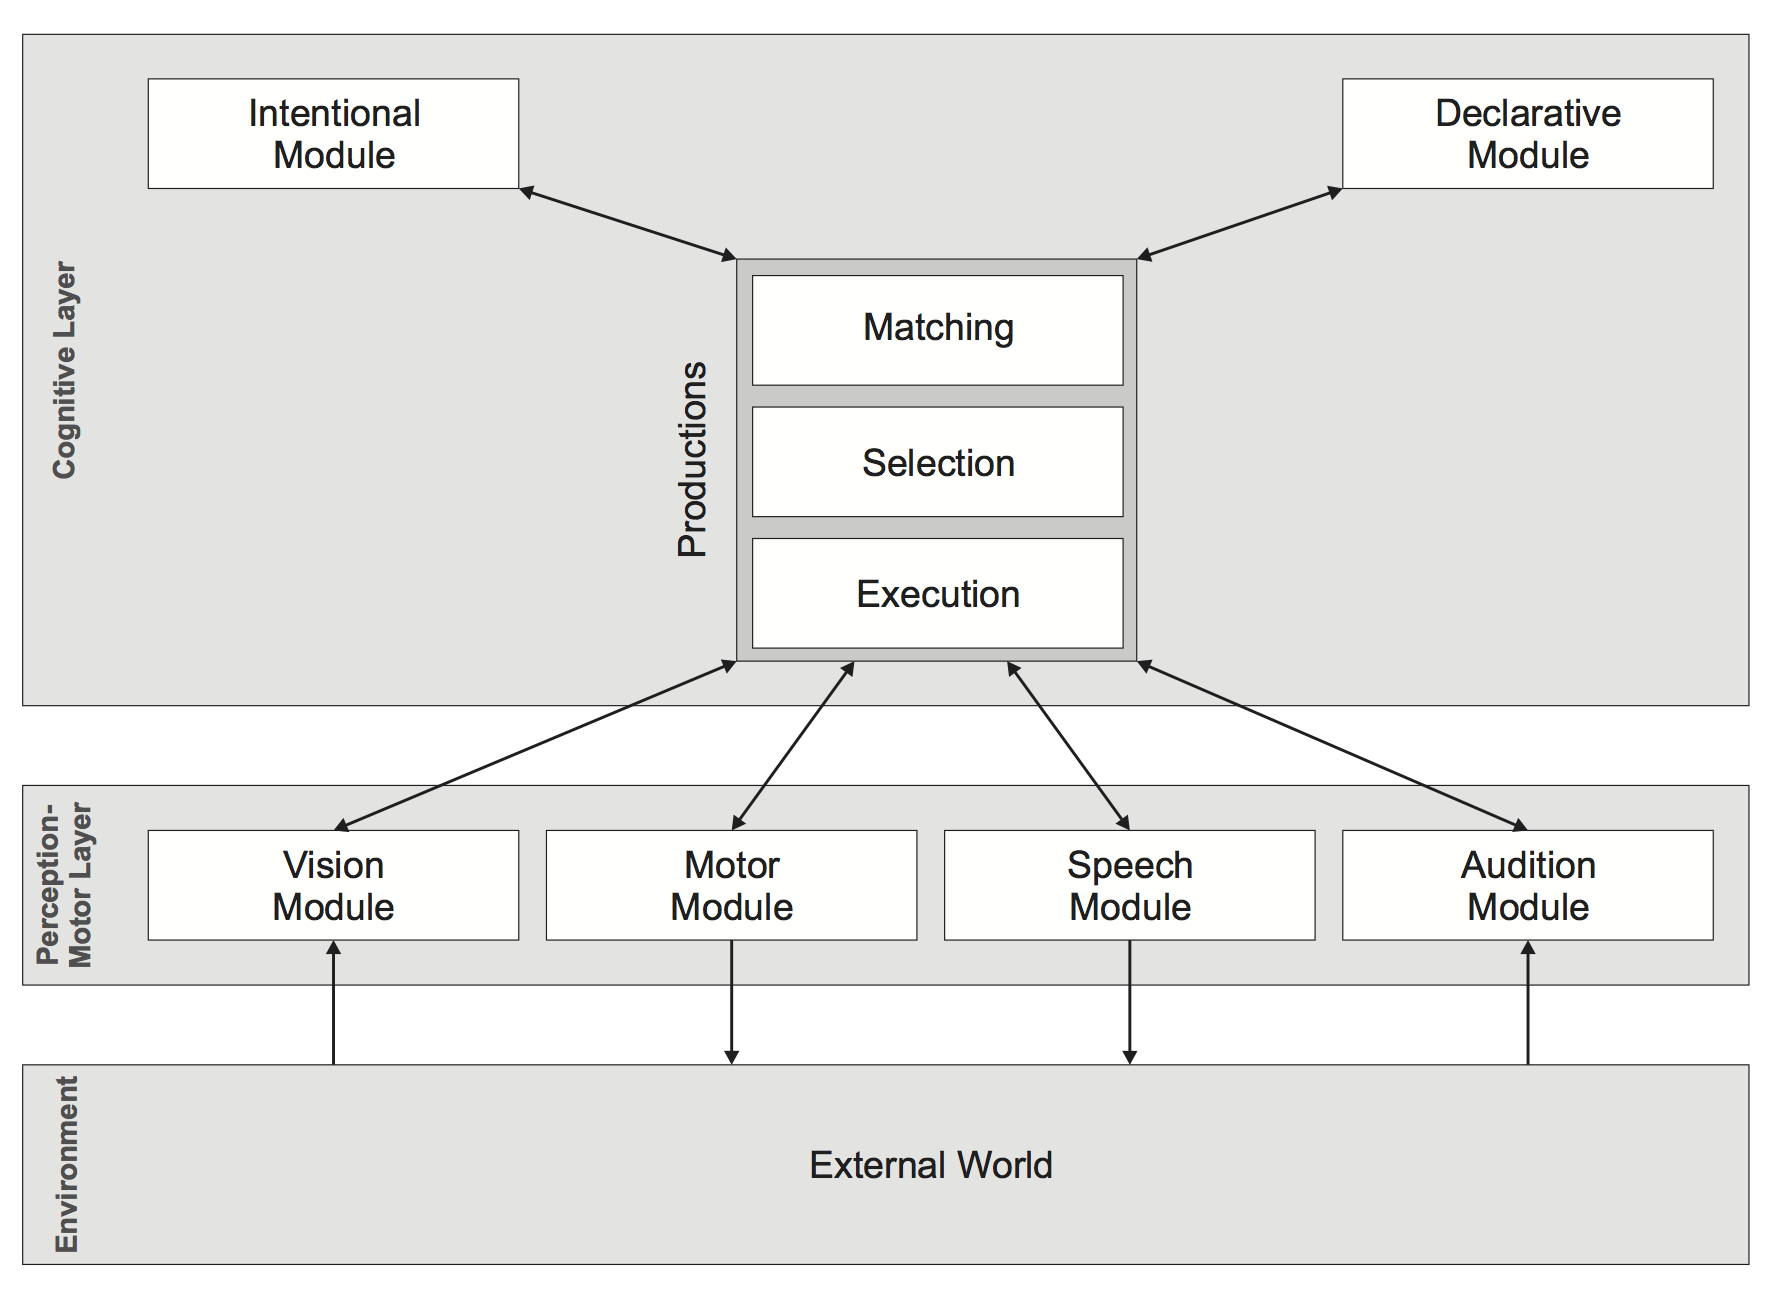
\includegraphics[width=0.85\textwidth]{act_r.png}
    \caption{Overview of the ACT-R high level architecture (from \cite{actr_4}).}
    \label{fig:act_r_1}
\end{figure}

The architecture can be generally described as two distinct layers: a \textit{perceptual-motor} layer and a \textit{cognitive} layer, as presented in Figure~\ref{fig:act_r_1}. The perceptual-motor layer corresponds to the interface of the cognition with the environment (which plays a key role in ACT-R), being comprised of modules such as vision and motor actions. The cognitive layer is focused on memory, which can be divided into two different categories: \textit{declarative} (consisting of factual knowledge and goals - e.g. \textit{"The maximum driving speed in a typical UK motorway is 70 mph"} or \textit{"Try get to point B"}) and \textit{procedural} (consisting of rules/procedures - e.g. \textit{"If the lead vehicle is going slowly, attempt an overtake"}) \cite{actr_4}. Furthermore, declarative memory is composed of \textit{chunks}, which are smaller pieces of information, divided into categories and attributes, that form more complex memories. In the example \textit{"The maximum driving speed in a typical UK motorway is 70 mph"}, \texttt{maximum driving speed in a typical UK motorway} is a category, whereas \texttt{70 mph} is an attribute. Another possible attribute for this category could be \texttt{113 km/h} (since $70 mph \simeq 113 km/h$).

\section{Integrated Driver Modelling in ACT-R}
\label{sec:salvucci}

The human driver model Salvucci introduced in \cite{salvucci_1} was developed with a specific scenario in mind: \textit{"(...) driving a standard midsize vehicle on a multilane highway with moderate traffic"} \cite{salvucci_1}. It consists of three distinct modules interacting in a sequential way: \textbf{control}, \textbf{monitoring}, and \textbf{decision making}. A high level schematic of the model can be found in Figure~\ref{fig:high_level_salvucci}.

\vspace{1em}
\begin{figure}[h]
    \centering
    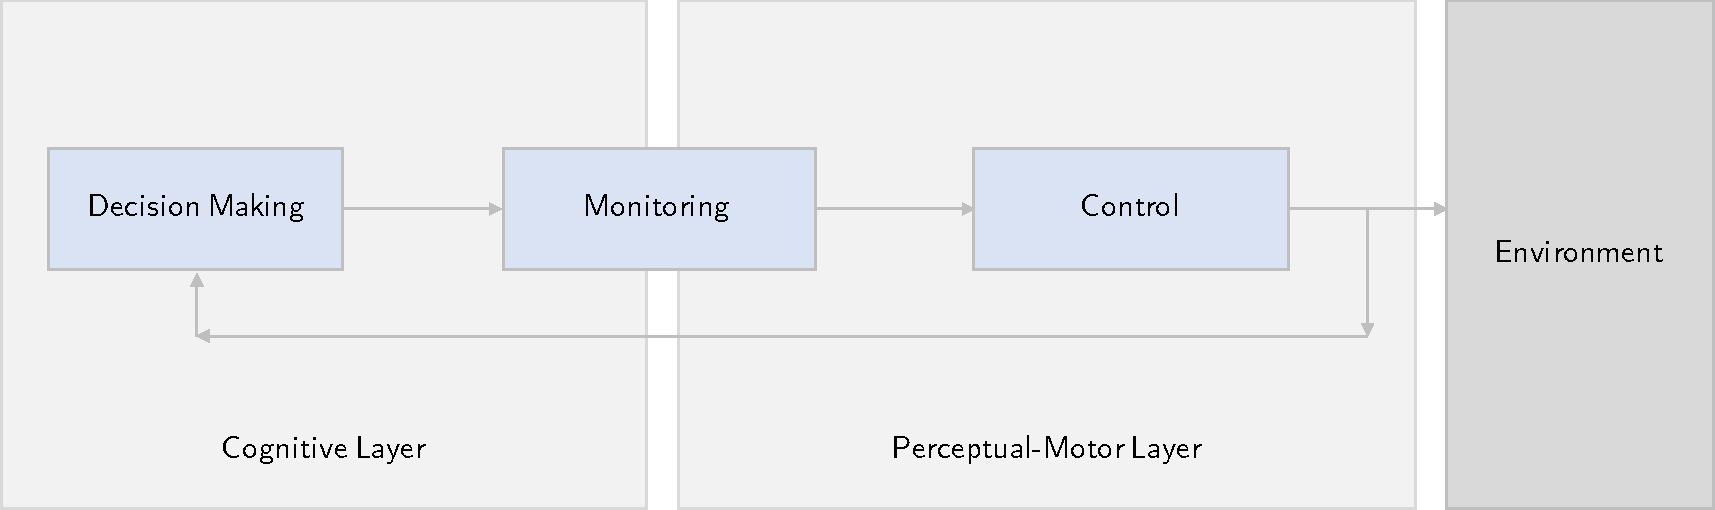
\includegraphics[width=1\textwidth]{high_level_salvucci.pdf}
    \caption{High level representation of the architecture presented in \cite{salvucci_1}.}
    \label{fig:high_level_salvucci}
\end{figure}

The \textbf{control} component manages both the lower level perception cues and the physical manipulation of the vehicle (e.g. steering, accelerating or breaking). The module can be divided into lateral (i.e. steering) and longitudinal (i.e. velocity) control, each modelled by a separate control law. 

The lateral control is determined by the existence of two artefacts that the driver obtains using lower level perception cues: the \textit{near point} and the \textit{far point}. In this model,  \textit{"the near point represents the vehicle’s current lane position, used to judge how close the vehicle is to the center of the roadway (...) [and] is characterized as a point in the center of the near lane visible in front of the vehicle, set at a distance of 10 m from the vehicle’s center"} while \textit{"the far point indicates the curvature of the upcoming roadway, used to judge what the driver should execute to anticipate the upcoming curvature and remain in the current lane"} \cite{salvucci_1}. At any cycle $i > 0$, the model works by using perception to determine the visual angles $\theta_{near}^{(i)}$ and $\theta_{far}^{(i)}$ and calculates:

\begin{equation}
\begin{split}
	\Delta \theta_{near} & = \theta_{near}^{(i)} - \theta_{near}^{(i-1)} \\
	\Delta \theta_{far} & = \theta_{far}^{(i)} - \theta_{far}^{(i-1)}
\end{split}
\end{equation}

The control law for the steering angle $\varphi$ can be defined as:

\begin{equation}
	\Delta \varphi = k_{far} \Delta \theta_{far} + k_{near} \Delta \theta_{near} + k_I \min{(\theta_{near}^{(i)}, \theta_{\max})} \Delta t
\end{equation}

with $k_{far}$, $k_{near},k_{I}$ and $\theta_{\max}$ defined as in \cite{salvucci_1}.

The process for the longitudinal control is very similar. At any cycle $i > 0$, the model starts by encoding the position of the lead vehicle and calculating the time headway $thw_{car}^{(i)}$ to it. It then computes:

\begin{equation}
	\Delta thw_{car} = thw_{car}^{(i)} - thw_{car}^{(i-1)}
\end{equation}

The control law for the linear acceleration $\psi$ can be written as:

\begin{equation}
	\Delta \psi = k_{car} \Delta thw_{car} + k_{follow} (thw_{car} - thw_{follow})\Delta t
\end{equation}

with $k_{car}$, $k_{follow}$ and $thw_{follow}$ defined as in \cite{salvucci_1}.

These control laws can be applied in order to model the behaviour of the driver in terms of lane keeping and curve negotiation, and generalise to lane changing actions in a straightforward manner. In order to initiate a lane change, the driver just starts following the near and far points of the destination lane instead of the current lane, as Salvucci and Liu presented in \cite{older_3}.

The \textbf{monitoring} component maintains situational awareness through the awareness of the position of other vehicles around the driver's vehicle. It accomplishes this through a random-sampling, with probability $p_{monitor}$, of one of four areas: either the left or right lane, and either forward or backward (with equal probability). After deciding which area to sample (if any), the model uses visual perception to determine whether a vehicle is present or not. If it is, the distance, lane and direction are saved in ACT-R's declarative memory. The value of $p_{monitor}$ is defined in \cite{salvucci_1}.

Finally, the \textbf{decision making} module uses the information gathered in the monitoring and control stage (if any is available) to determine which tactical decision should be taken. In this model, the decision corresponds to determining when and where a lane change should occur. Salvucci describes this process in \cite{salvucci_1} as: \textit{"If the driver’s vehicle is in the right lane, the model checks the current time headway to the lead vehicle (if any); if the lead car time headway drops below a desired time headway $thw_{pass}$, the model decides to change lanes to pass the vehicle. If the driver vehicle is in the left lane, the model checks instead simply for the presence of a lead vehicle. If there is a lead vehicle, the model remains in the left lane (because this vehicle is also passing other vehicles); otherwise it decides to [try to] change lanes to return to the right lane"}. This process is summarised in the flowchart presented in Figure~\ref{fig:flowchart_dm}, and the value of $thw_{pass}$ is defined in \cite{salvucci_1}.

Even after this decision to change lanes is taken, the model must then determine whether it is actually safe to do so. In order to verify that it is, the model initially attempts to recall, from the declarative memory, the nearest vehicle to it in the destination lane. If one is recalled at a distance closer than $d_{safe}$, then the change is aborted. If not, then the vehicle performs a safety monitoring of the destination lane. If this monitoring does not observe a vehicle at a distance closer than $d_{safe}$, then the vehicle initiates the execution of the lane change. The parameter $d_{safe}$ is as defined in \cite{salvucci_1}.

\begin{figure}[H]
    \centering
    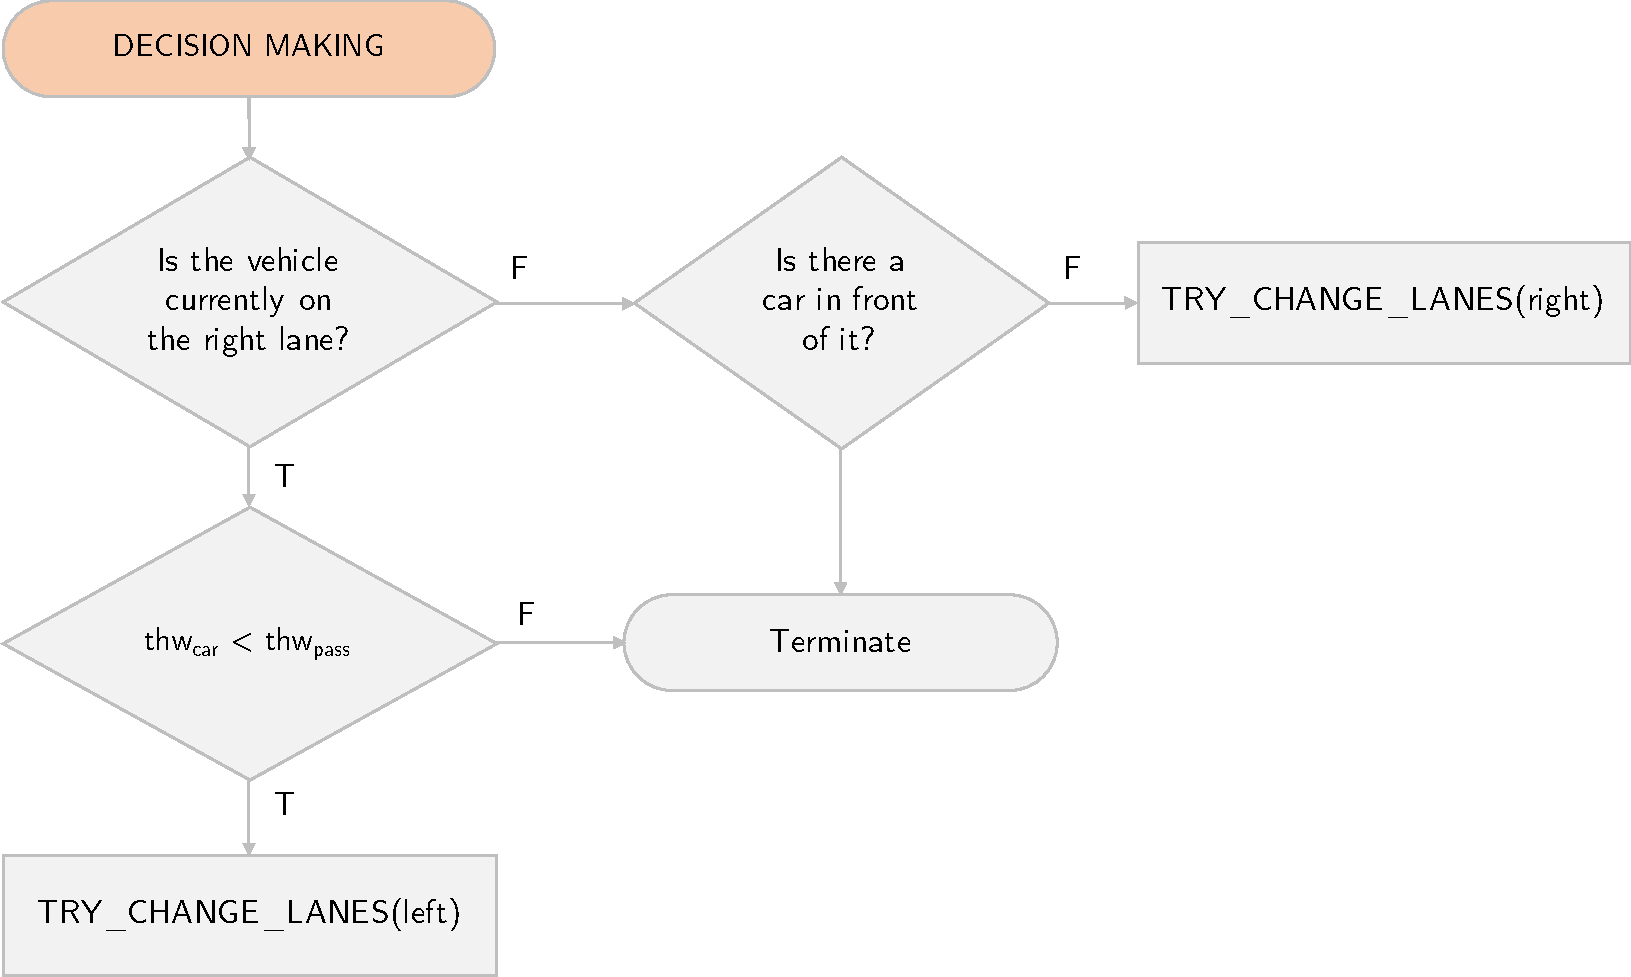
\includegraphics[width=1\textwidth]{flowchart_dm.pdf}
    \caption{Flowchart of part of the decision making process of the model.}
    \label{fig:flowchart_dm}
\end{figure}

\section{Probabilistic Model Checking}

Model checking is a formal verification technique consisting of the process of automatically verifying, through exhaustive search, whether a model meets a given specification \cite{bk08}. A model in this context is considered to be a labelled finite state-transition system, with states corresponding to configurations of the system and transitions between states representing the evolution between the said configurations.

Probabilistic model checking is a generalisation of model checking for the automated verification of systems that exhibit probabilistic behaviour \cite{fknp11, bk08}. It should be noted that this is not to be confused with \textit{probabilistic verification}, which amounts to partial state-space exploration \cite{bk08}. Within this section, important concepts of probabilistic model checking related to modelling of systems, and verification and synthesis of models will be explained in detail.

\subsection{Markov Chains and Decision Processes}
\label{sec:dtmcs_mdps}

Probabilistic model checking begins with the appropriate modelling of the system in a stochastic finite state-transition representation. There are several ways to do this according to the type of system to be modelled. 

In \textit{discrete-time Markov Chains} (DTMCs), all choices (i.e. transitions) are probabilistic \cite{bk08}. While this is useful in some cases, others require nondeterminism, which is where \textit{Markov Decision Processes} (MDPs) come in. In MDPs, nondeterministic probabilistic choices coexist. Essentially, a DTMC is an MDP with a uniquely determined probability distribution \cite{bk08}. Both DTMCs and MDPs can be augmented with reward structures, which correspond to real positive values assigned to states, transitions or actions that can be interpreted as bonuses or costs \cite{bk08}.

The formal definitions of DTMCs, MDPs and reward structures follow (adapted from \cite{bk08, fknp11, kp07}).

{\begin{defi}
{\vspace{1em}
\textbf{Discrete-time Markov Chain (DTMC)}}
{

A \textit{discrete-time Markov chain} is a tuple $\mathcal{M} = (S, \mathbf{P}, p_{init}, AP, L)$ such that:
\begin{itemize}
	\item $S$ is a countable, non-empty set of states
	\item $\mathbf{P}: S \times S \to [0,1]$ is a transition probability function such that for all states $s \in S$:
		\begin{equation}
			\sum_{s' \in S} \mathbf{P}(s,s') = 1
		\end{equation}
	\item $p_{init}: S \to [0,1]$ is the initial state distribution, such that:
		\begin{equation}
			\sum_{s \in S} p_{init}(s) = 1
		\end{equation}
	\item $AP$ is a set of atomic propositions, and 
	\item $L: S \to 2^{AP}$ is a labelling function. 
\end{itemize}

$\mathcal{M}$ is denoted \textit{finite} if $S$ and $AP$ are finite sets.
}
\end{defi}}

{\begin{defi}
\vspace{1em}
\textbf{Markov Decision Process (MDP)}
{

A \textit{Markov decision process} is a tuple $\mathcal{M} = (S, Act, \mathbf{P}, p_{init}, AP, L)$ such that:
\begin{itemize}
	\item $S$ is a countable, non-empty set of states
	\item $Act$ is a set of actions
	\item $\mathbf{P}: S \times Act \times S \to [0,1]$ is a transition probability function such that for all states $s \in S$ and actions $\alpha \in Act$:
		\begin{equation}
			\sum_{s' \in S} \mathbf{P}(s,\alpha,s') \in \{0,1\}
		\end{equation}
	\item $p_{init}: S \to [0,1]$ is the initial state distribution, such that:
		\begin{equation}
			\sum_{s \in S} p_{init}(s) = 1
		\end{equation}
	\item $AP$ is a set of atomic propositions, and
	\item $L: S \to 2^{AP}$ is a labelling function. 
\end{itemize}

An action $\alpha \in Act$ is enabled in a state $s$ if, and only if, $\sum_{s' \in S} \mathbf{P}(s,\alpha,s') = 1$. Let $Act(s)$ denote the set of actions enabled in a state $s$. It must be that for all states $s \in S$, $Act(s) \neq \emptyset$.
}
\end{defi}}

{\begin{defi}
\vspace{1em}
\textbf{Reward Structures for DTMCs and MDPs}
{

A \textit{reward structure} for a discrete-time Markov chain $\mathcal{M} = (S, \mathbf{P}, p_{init}, AP, L)$ is a tuple $\mathcal{C} = (\rho, \iota)$ such that:
\begin{itemize}
	\item $\rho: S \to \mathbb{R}_{\geq 0}$ is a state reward function
	\item $\iota: S \times S \to \mathbb{R}_{\geq 0}$ is a transition reward function
\end{itemize}
	
A \textit{reward structure} for a Markov decision process $\mathcal{M} = (S, Act, \mathbf{P}, p_{init}, AP, L)$ is a tuple $\mathcal{C} = (\rho, \iota)$ such that:
\begin{itemize}
	\item $\rho: S \to \mathbb{R}_{\geq 0}$ is a state reward function
	\item $\iota: S \times Act \to \mathbb{R}_{\geq 0}$ is an action reward function
\end{itemize}
}
\end{defi}}

There are some additional concepts related to DTMCs and MDPs which are relevant to the understanding of temporal logics and model checking. These are the concepts of paths in Markov chains or decision processes, and adversary in a Markov decision process (adapted from \cite{bk08, fknp11}).

{\begin{defi}
\vspace{1em}
\textbf{Paths in DTMCs and MDPs}
{

An \textit{(infinite) path} $\pi$ in a discrete-time Markov chain $\mathcal{M} = (S, \mathbf{P}, p_{init}, AP, L)$ is defined as an infinite sequence of states $\pi = s_0 \to s_1 \to s_2 ...$ (also written as $\pi = s_0s_1s_2...$) such that $\forall i \geq 0: \mathbf{P}(s_i, s_{i+1}) > 0$.

A \textit{finite path} $\rho$ in the discrete-time Markov chain $\mathcal{M}$ is defined as the prefix of an infinite path $\pi$, $\rho = s_0 \to s_1 \to ... \to s_n$ for $n > 0$.

An \textit{(infinite) path} $\pi$ in a Markov decision process $\mathcal{M} = (S, Act, \mathbf{P}, p_{init}, AP, L)$ is defined as an infinite sequence of states and actions $\pi = s_0 \xrightarrow{a_0} s_1 \xrightarrow{a_1} s_2 ...$ (also written as $\pi = s_0a_0s_1a_1s_2...$) such that $\forall i \geq 0: \mathbf{P}(s_i, a_i, s_{i+1}) > 0$.

A \textit{finite path} $\rho$ in the Markov decision process $\mathcal{M}$ is defined as the prefix of an infinite path $\pi$, $\rho = s_0 \xrightarrow{a_0} s_1 \xrightarrow{a_1} ... \xrightarrow{a_{n-1}} s_n$ for $n > 0$.

In both Markov chains and decision processes, the set of all infinite paths is denoted by $Paths(\mathcal{M})$, while the set of finite paths is denoted by $Paths_{fin}(\mathcal{M})$
}
\end{defi}}

{\begin{defi}
\vspace{1em}
\textbf{Adversary (alternatively Strategy or Scheduler)}
{

An \textit{adversary} for an MDP $\mathcal{M} = (S, Act, \mathbf{P}, p_{init}, AP, L)$ is a function $\sigma: S^+ \to Act$ such that $\sigma(s_0s_1...s_n) \in Act(s_n)$ for all $s_0s_1...s_n \in S^+$.

An adversary $\sigma$ is called memoryless if, and only if, for any $\pi_1 = s_0s_1...s_n$ and $\pi_2 = s'_0s'_1...s_n$ it is true that $\sigma(\pi_1) = \sigma(\pi_2) = \sigma(s_n)$.
}
\end{defi}}

\subsection{Temporal Logics}
\label{sec:temp_logics}

In order to verify properties in models, there needs to be a way of expressing those properties formally and unequivocally. While some reachability and reward-based properties come directly from the definition of DTMCs, MDPs and reward structures \cite{fknp11}, more interesting and complex properties require the use of a temporal logic. A propositional temporal logic is essentially an extension of propositional logic by temporal operators \cite{bk08}. In this context, one can consider time as being \textit{linear} or \textit{branching}. In linear time, at every moment in time there must only exist a single successor moment, whereas from the branching perspective, there may exist multiple ones, forming a tree-like structure of alternatives. Linear Temporal Logic (LTL) is a temporal logic which assumes the first, while Computation Tree Logic (CTL) is based on the branching perspective. Probabilistic Computational Tree Logic (PCTL) is an extension of CTL that takes into account a probabilistic operator.

Given the definition of a path in a MC and an MDP, it is possible to define the syntax and semantics of LTL and PCTL, as shown below (adapted from \cite{bk08, fknp11}).

{\begin{defi}
{\vspace{1em}
\textbf{Syntax and Semantics of LTL}}
{

An \textit{LTL formulae} $\varphi$ over a set of atomic propositions $AP$ can formed according to the following grammar:

\begin{equation}
	\varphi ::= \text{\texttt{true}} \bigmid a \bigmid \varphi_1 \wedge \varphi_2 \bigmid \neg \varphi \bigmid \text{X} \varphi \bigmid \varphi_1 \text{ U } \varphi_2
\end{equation}

where $a \in AP$, $\varphi_i$ are path formulas, X is the next operator and U is the until operator as defined below for Markov chains and decision processes.

For a given path $\pi = s_0s_1s_2...$ in a discrete-time Markov chain $\mathcal{M} = (S, \mathbf{P}, p_{init}, AP, L)$ (generalising trivially to a Markov decision process):
\begin{itemize}
	\item $\pi \models $\texttt{true} always.
	\item $\pi \models a$ if, and only if, $a \in L(s_0)$.
	\item $\pi \models \varphi_1 \wedge \varphi_2$ if, and only if, $\pi \models \varphi_1 \wedge \pi \models \varphi_2$.
	\item $\pi \models \neg \varphi$ if, and only if, $\pi \not\models \varphi$.
	\item $\pi \models \text{X}\varphi$ if, and only if, $s_1s_2... \models \varphi$.
	\item $\pi \models \varphi_1\text{ U }\varphi_2$ if, and only if:
	 \begin{equation}
	 	\exists i \geq 0 \text{ s.t. } (s_is_{i+1}... \models \varphi_2) \wedge (\forall j < i: s_js_{j+1}... \models \varphi_1)
	\end{equation}
\end{itemize}

The operator F (eventually) can also be defined as:

\begin{equation}
	\text{F} \varphi = \text{\texttt{true}} \text{ U } \varphi
\end{equation}

}
\end{defi}}

It can be noticed that, as a result of the linear time consideration in LTL, all the formulas are taken over paths. This is not the case in PCTL which can have both path and state formulae, as shown below.

%{\begin{defi}
%{\vspace{1em}
%\textbf{Syntax and Semantics of CTL}}
%{
%
%A \textit{CTL state formulae} $\Phi$ over a set of atomic propositions $AP$ can formed according to the following grammar:
%
%\begin{equation}
%	\Phi ::= \text{\texttt{true}} \bigmid a \bigmid \Phi_1 \wedge \Phi_2 \bigmid \neg \Phi \bigmid \text{E} \varphi \bigmid \text{A} \varphi
%\end{equation}
%
%where $a \in AP$, $\varphi$ is a path formula, $\Phi_i$ are state formulas, E is the exists operator, and A is the all operator as defined below for Markov chains and decision processes.
%
%For a given state $s \in S$ in a discrete-time Markov chain $\mathcal{M} = (S, \mathbf{P}, p_{init}, AP, L)$ (generalising trivially to a Markov decision process):
%\begin{itemize}
%	\item $s \models $\texttt{true} always.
%	\item $s \models a$ if, and only if, $a \in L(s)$.
%	\item $s \models \Phi_1 \wedge \Phi_2$ if, and only if, $s \models \Phi_1 \wedge s \models \Phi_2$.
%	\item $s \models \neg \Phi$ if, and only if, $s \not\models \Phi$.
%	\item $s \models \text{E} \varphi$ if, and only if, $\exists \pi \in Paths(s): \pi \models \varphi$.
%	\item $s \models \text{A} \varphi$ if, and only if, $\forall \pi \in Paths(s): \pi \models \varphi$
%\end{itemize}
%
%A \textit{CTL path formulae} $\varphi$ over a set of atomic propositions $AP$ can formed according to the following grammar:
%
%\begin{equation}
%	\varphi ::= \text{X} \Phi \bigmid \Phi_1 \text{ U } \Phi_2
%\end{equation}
%
%where $a \in AP$, $\Phi_i$ are state formulas, X is the next operator, and U is the until operator as defined below for Markov chains and decision processes.
%
%For a given path $\pi = s_0s_1s_2...$ in a Markov chain $\mathcal{M} = (S, \mathbf{P}, p_{init}, AP, L)$ (generalising trivially to a Markov decision process):
%\begin{itemize}
%	\item $\pi \models \text{X}\Phi$ if, and only if, $s_1 \models \Phi$.
%	\item $\pi \models \Phi_1\text{ U }\Phi_2$ if, and only if:
%	 \begin{equation}
%	 	\exists i \geq 0 \text{ s.t. } (s_i \models \Phi_2) \wedge (\forall j < i: s_j \models \Phi_1)
%	\end{equation}
%\end{itemize}
%
%It is also possible to define the operators F (eventually) and G (globally) as:
%
%\begin{equation}
%\begin{aligned}
%	\text{F} \Phi & = \text{\texttt{true}} \text{ U } \Phi \\
%	\text{G} \Phi & = \neg \text{E} (\neg \Phi)
%\end{aligned}
%\end{equation}
%
%}
%\end{defi}}

{\begin{defi}
{\vspace{1em}
\textbf{Syntax and Semantics of PCTL}}
{

A \textit{PCTL state formulae} $\Phi$ over a set of atomic propositions $AP$ can formed according to the following grammar:

\begin{equation}
	\Phi ::= \text{\texttt{true}} \bigmid a \bigmid \Phi_1 \wedge \Phi_2 \bigmid \neg \Phi \bigmid \mathbb{P}_{\triangleright p} (\varphi)
\end{equation}

where $a \in AP$, $\Phi_i$ are state formulas, $\varphi$ is a path formula, $p \in [0,1]$, $\triangleright \in \{>, <, \geq, \leq\}$ is a probability bound, and $\mathbb{P}_{\triangleright p}$ is the probabilistic operator as defined below for Markov chains and decision processes.

For a given state $s \in S$ in a discrete-time Markov chain $\mathcal{M} = (S, \mathbf{P}, p_{init}, AP, L)$ (generalising trivially to a Markov decision process):
\begin{itemize}
	\item $s \models $\texttt{true} always.
	\item $s \models a$ if, and only if, $a \in L(s)$.
	\item $s \models \Phi_1 \wedge \Phi_2$ if, and only if, $s \models \Phi_1 \wedge s \models \Phi_2$.
	\item $s \models \neg \Phi$ if, and only if, $s \not\models \Phi$.
	\item $s \models \mathbb{P}_{\triangleright p} (\varphi)$ if, and only if, $P_s (\pi \in Paths(s): \pi \models \varphi) \triangleright p$ (that is, the probability, from state $s$, that $\varphi$ is true for an outgoing path satisfies $\triangleright p$).
\end{itemize}

A \textit{PCTL path formulae} $\varphi$ over a set of atomic propositions $AP$ can formed according to the following grammar:

\begin{equation}
	\varphi ::= \text{X} \Phi \bigmid \Phi_1 \text{ U}^{\leq k}\, \Phi_2 \bigmid \Phi_1 \text{ U } \Phi_2
\end{equation}

where $a \in AP$, $k \in \mathbb{N}$, $\Phi_i$ are state formulas, X is the next operator, U is the until operator, and U$^{\leq k}$ is the bounded-until operator as defined below for Markov chains and decision processes.

For a given path $\pi = s_0s_1s_2...$ in a discrete-time Markov chain $\mathcal{M} = (S, \mathbf{P}, p_{init}, AP, L)$ (generalising trivially to a Markov decision process):
\begin{itemize}
	\item $\pi \models \text{X}\Phi$ if, and only if, $s_1 \models \Phi$.
	\item $\pi \models \Phi_1\text{ U}^{\leq k}\, \Phi_2$ if, and only if:
	 \begin{equation}
	 	\exists i \leq k \text{ s.t. } (s_i \models \Phi_2) \wedge (\forall j < i: s_j \models \Phi_1)
	\end{equation}
	\item $\pi \models \Phi_1\text{ U }\Phi_2$ if, and only if:
	 \begin{equation}
	 	\exists i \geq 0 \text{ s.t. } (s_i \models \Phi_2) \wedge (\forall j < i: s_j \models \Phi_1)
	\end{equation}
\end{itemize}

Similarly to CTL, it is possible to define the operators F (eventually) and G (globally) as:

\begin{equation}
\begin{aligned}
	\text{F} \Phi & = \text{\texttt{true}} \text{ U } \Phi \\
	\text{G} \Phi & = \neg \text{E} (\neg \Phi)
\end{aligned}
\end{equation}

}
\end{defi}}

While PCTL path formulas are defined above, it should be mentioned that all PCTL formulas are state formulas, and that path formulas should only appear inside the probabilistic operator. 

In relation to the probabilistic operator in PCTL, the generalisation from the Markov chain to the Markov decision process can be done using the concept of adversary (also denoted strategy or scheduler), initially introduced in Section~\ref{sec:dtmcs_mdps}. In the case of an MDP, the operator $\mathbb{P}_{\triangleright p}$ should be interpreted under the following semantics:

\begin{equation}
	s \models \mathbb{P}_{\triangleright p} (\varphi) \text{ if, and only if, } \forall \sigma \in Adv: Pr^{\sigma}_s (\pi \in Paths^{\sigma}(s): \pi \models \varphi) \triangleright p
\end{equation}

that is, the probability, from state $s$, that $\varphi$ is true for an outgoing path satisfies $\triangleright p$ for all adversaries $\sigma \in Adv$ (with $Adv$ constituting the set of all adversaries that the MDP admits).

\subsection{PRISM Language}

PRISM is a probabilistic model checking tool developed in cooperation between the Universities of Oxford and Birmingham \cite{prism}. It was one of the first tools within stochastic model checking to be released and its development is currently headed by David Parker. In order to use PRISM (and other alternative model checking tools), it is essential to be able to specify the model. To achieve this, the team behind PRISM developed the PRISM Language, initially described in \cite{prism_1}.

A model described in PRISM Language (typically a \texttt{.pm}, \texttt{.nm} or \texttt{.prism} text file) should contain a keyword that indicates the kind of model to expect. For example, the keyword \texttt{dtmc} indicates the model is a DTMC (discrete-time Markov chain) and \texttt{mdp} indicates a MDP (Markov decision process).

PRISM Language uses two different basic components to define a model: \textit{modules} and \textit{variables}. A module is composed of a set of local variables whose behaviour is described by \textit{commands}. A general command is of the form:

{\vspace{1em}
\begin{lstlisting}
[] guard -> prob_1: update_1 + ... + prob_n: update_n;
\end{lstlisting}
}

where \textit{guard} is a boolean expression over the variables, \textit{prob\_i} is the probability that \textit{update\_i} will be taken (with $\sum_i \text{prob\_i} = 1$) and \textit{update\_i} is the new value the local and/or global variables take if the guard is true and a transition is taken to this configuration.

A state of the module is defined as a configuration of its local variables, and a state of the model is a configuration of the states of all modules which compose it and the global variables.

In Listing \ref{lst:example}, an example of a simple MDP model described in PRISM Language is shown. This example is comprised of two modules, \texttt{M1} and \texttt{M2}, each with their own local variables, and no global variables are declared. It should be noted that the variables in PRISM Language should either be integers (\texttt{int}) or booleans (\texttt{bool}) and can be initialised by specifying \texttt{init} after the initial declaration. Due to the fact that we are dealing with finite models, the integers must be in a finite range.

{\vspace{1em}
\begin{lstlisting}[caption={Example of a simple MDP model from \cite{prism_example} (modified)},captionpos=b,label={lst:example}]
// Example 1 (modified)
// Two process mutual exclusion

mdp

module M1

    x : [0..2] init 0;

    [] x=0 -> 0.8:(x'=0) + 0.2:(x'=1);
    [] x=1 & y!=2 -> (x'=2);
    [] x=2 -> 1:(x'=2);
    [] x=2 -> 1:(x'=0);

endmodule

module M2

    y : [0..2] init 0;

    [] y=0 -> 0.8:(y'=0) + 0.2:(y'=1);
    [] y=1 & x!=2 -> (y'=2);
    [] y=2 -> 1:(y'=2);
    [] y=2 -> 1:(y'=0);

endmodule
\end{lstlisting}
}

Models in the PRISM Language can also include \textit{formulas}, which are expressions that avoid repetition of code, and \textit{labels}, which are boolean expressions that identify sets of states of interest.

It is also possible to define rewards structures using the following convention:

\begin{minipage}{\linewidth}
{\vspace{1em}
\begin{lstlisting}
rewards "name"
    guard: state_reward;
    ...
    [action] guard: transition_reward;
    ...
endrewards
\end{lstlisting}
}
\end{minipage}

where the \textit{guards} are similarly defined as before, but the distinction between state and transition rewards is defined by the \textit{action} (which may be empty).

\subsection{Model Checking and Strategy Synthesis in DTMCs and MDPs}

After the description of the model using a language such as PRISM Language, it is possible to verify properties on the said model. These properties can be of different types according to the model and the model checking tool chosen. 

In this dissertation, the models built will be represented through discrete-time Markov chains and Markov decision processes, so the properties of interest tend to be best expressed in the temporal logics LTL or PCTL. The PRISM model checker allows a user to import a text file with the probabilistic model, build it and verify LTL and PCTL properties on it \cite{prism}. Another tool used for this purpose is the Storm model checker \cite{storm}. Each of these tools has it strengths and weaknesses. PRISM is an extremely robust tool, with lots of options in terms of engines to perform the required calculations, and a graphical interface. Storm is a relatively recent tool which builds on top of some of PRISM's features and introduces new ones, such as an optimised Sparse engine (a great advantage when dealing with models with a small state space) and conditional properties in DTMCs \cite{storm}. However, it does not provide a graphical interface and is limited in terms of capabilities and I/O. Due to the fact that Storm builds on top of PRISM, it allows models described in PRISM Language as input and the properties are specified using the same convention.

In order to illustrate properties, consider the example of Listing~\ref{lst:example}. A PCTL property in this case could be defined as:

\begin{minipage}{\linewidth}
{\vspace{1em}
\begin{lstlisting}
P>=0.5 [F x = 2]
\end{lstlisting}
}
\end{minipage}

This property can be interpreted as \textit{"with probability greater or equal to 0.5, eventually the model reaches a state where }\texttt{x = 2}\textit{"}. Building the model and verifying the property yields the value \texttt{false}, which means that, according to this model, there exists at least one adversary under which this property is not satisfied. Both PRISM and Storm allow for quantitative probabilistic properties as well. These properties take different formats in DTMCs and MDPs, as presented below.

\begin{minipage}{\linewidth}
{\vspace{1em}
\begin{lstlisting}
// DTMC
P=? [F x = 2]

// MDP
Pmin=? [F x = 2]
Pmax=? [F x = 2]
\end{lstlisting}
}
\end{minipage}

Instead of returning a boolean value of satisfaction, these return the actual values of the probabilities of the properties being satisfied. They are, therefore, extremely useful metrics for model comparison. For the case of the DTMC, due to the fact that there is no nondeterminism, the probability of a path is uniquely defined (as seen in Section~\ref{sec:temp_logics}), and thus can be expressed simply using the operator \texttt{P=?}. For MDPs, this is not the case. In order to verify the probabilistic operator $\mathbb{P}_{\triangleright p}$ on the path formula $\varphi$, a model checker needs to calculate the following quantities:

\begin{equation}
\begin{aligned}
	p_{\max, s} (\varphi) & = \sup_{\sigma \in Adv} P^{\sigma}_s (\varphi) \\
	p_{\min, s} (\varphi) & = \inf_{\sigma \in Adv} P^{\sigma}_s (\varphi)
\end{aligned}
\end{equation}

where $P^{\sigma}_s (\varphi) = Pr^{\sigma}_s (\pi \in Paths^{\sigma}(s): \pi \models \varphi)$.

Therefore, PRISM and Storm allow users to access these values by writing properties using \texttt{Pmax} and \texttt{Pmin} (boolean or quantitative). 

Storm allows for conditional probability properties of the type:

\begin{minipage}{\linewidth}
{\vspace{1em}
\begin{lstlisting}
P=? [ F x=2 || F y=2 ]
\end{lstlisting}
}
\end{minipage}

This property can be interpreted as \textit{"what is the probability that the model eventually reaches the state} \texttt{x = 2}\textit{, given that it eventually reaches the state} \texttt{y = 2}\textit{"}. These properties, in DTMCs, correspond simply to the application of Bayes' theorem of conditional probability, which states that:

\begin{equation}
	P_s (\varphi_1 \cond \varphi_2) = \frac{P_s (\varphi_1 \wedge \varphi_2)}{P_s (\varphi_2)}
\end{equation}

For $P_s (\varphi_2) \neq 0$. 

\textbf{Note}: while uncommon in mathematical notation, the event \textit{"A conditioned on B"} will be represented throughout the dissertation by $A \cond B$, so as to be distinguishable from the boolean disjunction operator which is represented as $A\mid B$ (reads \textit{"A or B"}).

It must be emphasised that this is \textbf{not} the case for MDPs, where the existence of multiple adversaries complicates the calculations of conditional probabilities. Despite this, \cite{cond_prob} presents a polynomial-time algorithm for computing conditional properties in MDPs which is yet to be implemented in any model checking tool.

This does not mean that it is not possible to reason over conditional probabilities in MDPs. For some specific scenarios, it is possible to obtain meaningful bounds which allow comparisons between the ones obtained in DTMCs and MDPs. One of those scenarios is defined in the proposition below, with the proof following it.

\begin{proposition}
\label{pro:cond_props}
Consider a Markov decision process $\mathcal{M} = (S, Act, \mathbf{P}, p_{init}, AP, L)$ which admits adversaries $\sigma \in Adv$. Let $\varphi_1, \varphi_2$ be two PCTL path formulas, such that, for any path $\pi \in Paths(s)$: $\pi \models \varphi_1 \Rightarrow \pi \models \varphi_2$. Assume as well that:

\begin{equation}
	\sigma' \in \arg\sup_{\sigma \in Adv} P^{\sigma}_s (\varphi_1 \cond \varphi_2)
\end{equation}

And that:

\begin{equation}
	P^{\sigma'}_s (\varphi_1) = p_{\max, s} (\varphi_1)
\end{equation}

That is, an adversary which maximises the probability of $\varphi_1 \bigmid \varphi_2$ also maximises the probability of $\varphi_1$. In this case it holds that:

\begin{equation}
	p_{\max, s} (\varphi_1 \cond \varphi_2) \geq \frac{p_{\max, s} (\varphi_1)}{p_{\max, s} (\varphi_2)}
\end{equation}

with:

\begin{equation}
	p_{\max, s} (\varphi_1 \cond \varphi_2) = \sup_{\sigma \in Adv} P^{\sigma}_s (\varphi_1 \cond \varphi_2)
\end{equation}

\end{proposition}
 
\begin{proof}
%Consider that exists an adversary $\sigma'_1 \in Adv$, such that:

%\begin{equation}
%	p_{\max, s} (\varphi_1 \bigmid \varphi_2) < \frac{P^{\sigma'_1}_s (\varphi_1)}{P^{\sigma'_1}_s (\varphi_2)}
%\end{equation}

%We will prove that this leads to a contradiction.

Consider $\sigma_2 \in Adv$ such that:

\begin{equation}
\label{eq:max_sigmas}
	\sigma_2 \in \arg\sup_{\sigma \in Adv} P^{\sigma}_s (\varphi_2)
\end{equation}

Assume, for the sake of contradiction, that:

\begin{equation}
	p_{\max, s} (\varphi_1 \cond \varphi_2) < \frac{p_{\max, s} (\varphi_1)}{p_{\max, s} (\varphi_2)}
\end{equation}

Under adversary $\sigma'$, it can be written that, through Bayes' theorem of conditional probability:

\begin{equation}
	p_{\max, s} (\varphi_1 \cond \varphi_2) = P^{\sigma'} _s(\varphi_1 \cond \varphi_2) = \frac{P^{\sigma'}_s (\varphi_1 \wedge \varphi_2)}{P^{\sigma'}_s (\varphi_2)} = \frac{P^{\sigma'}_s (\varphi_1)}{P^{\sigma'}_s (\varphi_2)}
\end{equation}

Therefore, it follows that:

\begin{equation}
	\frac{P^{\sigma'}_s (\varphi_1)}{P^{\sigma'}_s (\varphi_2)} < \frac{p_{\max, s} (\varphi_1)}{p_{\max, s} (\varphi_2)}
\end{equation}

For this to be true, it must be that $P^{\sigma'}_s (\varphi_2) > p_{\max, s} (\varphi_2)$, since $P^{\sigma'}_s (\varphi_1) = p_{\max, s} (\varphi_1)$. This constitutes a contradiction, since in that case $\sigma_2$ would not maximise the probability of $\varphi_2$ ($p_{\max, s} (\varphi_2) = P^{\sigma_2}_s (\varphi_2)$, by definition), a violation of the assumption described in Equation~\ref{eq:max_sigmas}. Thus, the proposition is proven.
\end{proof}

In MDPs it is also possible to perform multi-objective verification, whereas multiple properties will be tested simultaneously (both in PRISM and Storm). One example of this would be:

\begin{minipage}{\linewidth}
{\vspace{1em}
\begin{lstlisting}
multi(P>=0 [F x=2], P>=0.2 [F y=2])
\end{lstlisting}
}
\end{minipage}

The value of the verification of this property corresponds to the boolean conjunction of the individual properties. It is also possible to optimise over a single property while constraining other properties, restricting the possibilities in terms of outcomes. An example of this would be:

\begin{minipage}{\linewidth}
{\vspace{1em}
\begin{lstlisting}
multi(Pmax=? [F x=2], P>=0.2 [F y=2])
\end{lstlisting}
}
\end{minipage}

Finally, it is also possible to perform multi-objective optimisation over the properties by defining them as (for example):

\begin{minipage}{\linewidth}
{\vspace{1em}
\begin{lstlisting}
multi(Pmax=? [F x=2], Pmax=? [F y=2])
\end{lstlisting}
}
\end{minipage}

This leads to a situation where compromises between the optimisation of either one of the properties might have to be reached. Pareto curves are the result of the verification of such properties and their formal definition is presented below (adapted from \cite{pareto}).

{\begin{defi}
{\vspace{1em}
\textbf{Multi-objective Query, Pareto Vector and Pareto Curve (alternatively Set)}}
{

A \textit{multi-objective query} (MQ) $\phi$ of $n$ objectives is a positive boolean combination of $n$ predicates of the form $r_i \geq v_i$, where $r_i$ is a reward function, $v_i \in \mathbb{Q}$ is a bound. The notation $\phi[\mathbf{x}]$, $\mathbf{x} \in \mathbb{R}^n$ is used to denote $\phi$ in which each $r_i \geq v_i$ is replaced by $r_i \geq x_i$

Consider a multi-objective query MQ $\phi$ of $n$ objectives. The vector $\mathbf{x} \in \mathbb{R}^n$ is a \textit{Pareto vector} of $\phi$ if, and only if:

\begin{enumerate}
	\item $\phi[\mathbf{x} - \varepsilon]$ is achievable for all $\varepsilon > 0$, and
	\item $\phi[\mathbf{x} + \varepsilon]$ is not achievable for any $\varepsilon > 0$
\end{enumerate}

A \textit{Pareto curve} of $\phi$ is the set of all Pareto vectors that $\phi$ admits.

}
\end{defi}}

Thus, the result of the verification of a multi-objective optimisation property corresponds to a Pareto curve (this curve might contain a single vector). Both PRISM and Storm allow for the verification of properties containing up to 2 objectives each. As a result, 2D plots are the best way to represent these solutions. In Figure~\ref{fig:pareto_1}, the result of the verification of the property \texttt{multi(Pmax=? [F G x=2], Pmax=? [F G y=2])} in the model described in Listing~\ref{lst:example} is shown. As it can be observed, either property can be satisfied with certainty, but not both simultaneously (mutual exclusion). The light green area under the curve corresponds to the achievable set.

\begin{figure}[h]
    \centering
    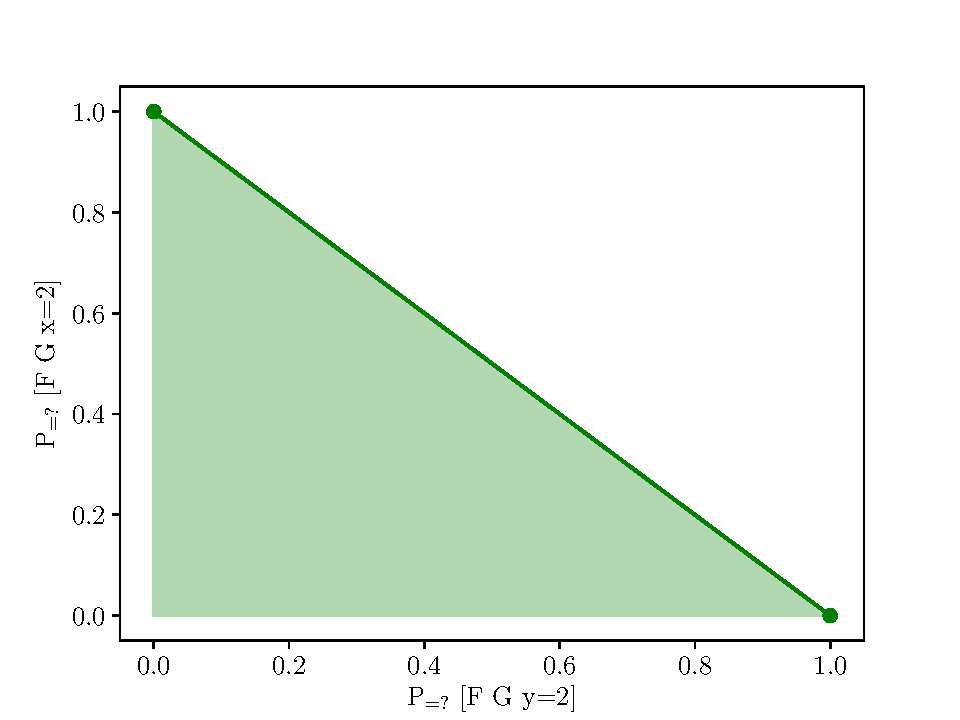
\includegraphics[width=0.9\textwidth]{pareto_1.pdf}
    \caption{Example of a Pareto curve represented as a 2D plot.}
    \label{fig:pareto_1}
\end{figure}

Each of the values resulting of the verification of quantitative properties in MDPs (whether they be a single value from a single-objective optimisation, or a Pareto vector) is the result of an adversary which solves the nondeterminism and converts the MDP into a DTMC \cite{bk08}. The process of obtaining the adversary which satisfies certain properties is denoted by \textbf{strategy synthesis} or \textbf{adversary generation}, and it is formally defined below.

{\begin{defi}
{\vspace{3em}
\textbf{Strategy Synthesis (alternatively Adversary Generation)}}
{

Consider a Markov decision process $\mathcal{M} = (S, Act, \mathbf{P}, p_{init}, AP, L)$. The process of maximal (similarly minimal) \textit{strategy synthesis} of the path formula $\varphi$ is defined as a process that yields an adversary $\sigma \in Adv$ such that:

\begin{equation}
	\sigma \in {\arg\sup}_{\sigma' \in Adv} P^{\sigma'}_s (\varphi)
\end{equation}

(respectively $\arg\inf$ for minimal), where $Adv$ is the set of all adversaries that $\mathcal{M}$ admits.

}
\end{defi}}

